\section{Разработка базы знаний и инструментов для работы с ней}
\label{sec:development}

\subsection{Выбор технологических средств реализации}

\subsubsection*{Языки, форматы, библиотеки и инструменты}

В качестве основы для представления и хранения знаний в проекте выбран документно-ориентированный полуструктурированный подход: содержательная часть единицы знаний оформляется в формате \textbf{Markdown} (.md), а машиночитаемые метаданные размещаются во фронтматтере на базе \textbf{YAML}. Для обмена данными через программные интерфейсы используется \textbf{JSON}. Классические онтологические форматы (RDF/RDFS/OWL), как и языки запросов к графовым структурам (SPARQL, Cypher), на данном этапе не задействуются, поскольку реализация строится поэтапно: в первую очередь требуется создать лёгкую, удобную для версионирования и коллективной разработки структуру, полностью совместимую с системами контроля версий.

В состав используемого инструментального стека входят:
\begin{itemize}
    \item \textbf{Python 3.12} — основной язык разработки CLI-средства и серверной части;
    \item \textbf{PyYAML 6.0.1} — библиотека обработки YAML-метаданных;
    \item \textbf{Pydantic v2.5} — средство строгой типизации, схемной валидации и сериализации JSON;
    \item \textbf{FastAPI 0.109.2 / Uvicorn 0.27.0} — стек для асинхронного HTTP-сервера веб-MVP;
    \item \textbf{Vanilla JS (ES6 modules)} — реализация клиентской части без использования тяжёлых фреймворков;
    \item \textbf{pytest 8.0.2} — фреймворк автоматизированного тестирования (177 тестов).
\end{itemize}

Фреймворки класса RAG (LangChain, LlamaIndex, Haystack), а также rule engines (Drools, CLIPS) в текущую версию прототипа не включены. При этом в серверной архитектуре (\texttt{server.py}) заранее предусмотрена точка расширения для подключения RAG-конвейера, помеченная комментарием \texttt{\# TODO: RAG INTEGRATION}.

\subsubsection*{Обоснование выбора средств}

Комбинация Markdown + YAML + Python выбрана исходя из особенностей предметной области и требований, предъявляемых к базе знаний. Такой стек позволяет совместить удобство восприятия для инженеров знаний с пригодностью к машинной обработке в автоматизированных конвейерах. YAML делает возможным строгую формализацию метаданных: идентификаторов, перечислимых полей, массивов связей и других структурированных атрибутов. Это снижает вероятность появления произвольных значений и упрощает контроль целостности. Markdown, в свою очередь, сохраняет гибкость представления инженерного содержания, включая ASCII-схемы, фрагменты кода и вложенные списки, что особенно важно для технических описаний.

Автоматический контроль корректности и вывод служебной информации реализованы в модулях \texttt{validator.py} и \texttt{registry.py}. Для проверки схем используется Pydantic, а формат идентификаторов дополнительно контролируется регулярными выражениями. Поисковые операции выполняются на этапе разбора фронтматтера, благодаря чему достигается интерактивное время отклика без необходимости развёртывания отдельной СУБД. Документно-файловая организация естественным образом поддерживается Git, что обеспечивает версионирование, совместную параллельную работу участников и автоматизируемый процесс ревью через Pull Request.

В дальнейшем выбранный формат допускает органичное расширение в сторону интеллектуальных модулей. YAML-метаданные могут быть сравнительно просто преобразованы в RDF/OWL при переходе к онтологическому представлению, а содержимое Markdown-документов уже пригодно для векторизации и разбиения на чанки при подключении RAG-конвейера (LangChain + ChromaDB/Qdrant).

\subsection{Реализация структуры и наполнения базы знаний}

Формирование базы знаний организовано по полуавтоматической схеме. В роли источников знаний используются фундаментальные учебные издания, официальная технологическая документация и заслуживающие доверия инженерные блоги. Критерии отбора материала включают обязательное соответствие целевому уровню сложности (Junior/Middle/Senior), фиксацию частоты появления темы на собеседованиях, а также подтверждение каждого факта как минимум одним авторитетным источником. Нормализация данных обеспечивается строгим соблюдением таксономии тегов и формата идентификаторов, зафиксированных в \texttt{\_meta/tag\_taxonomy.md} и \texttt{CONTRIBUTING.md}.

Добавление новых знаний выполняется через CLI-инструмент: команда \texttt{python3 main.py new} создаёт файл по шаблону с автоматически заполненными ID и обязательными полями. Далее инженер вручную дополняет содержательные разделы, переводит материал в состояние \texttt{review}, запускает команду \texttt{validate} и фиксирует изменения в Git. После проверки другим участником статус изменяется на \texttt{approved}.

Логическая модель (глобальный слой и три предметные области) на физическом уровне представлена файловой иерархией: \texttt{cs/}, \texttt{arch/}, \texttt{process/}, \texttt{global/}. Каждая единица знаний располагается в отдельном файле, имя которого формируется по шаблону \texttt{\{домен\}\_\{категория\}\_\{slug\}.md}. Связи между классами единиц знаний описываются в YAML-фронтматтере через массивы \texttt{related} и \texttt{prerequisites}, за счёт чего формируется ориентированный ациклический граф знаний.

\begin{figure}[H]
\centering
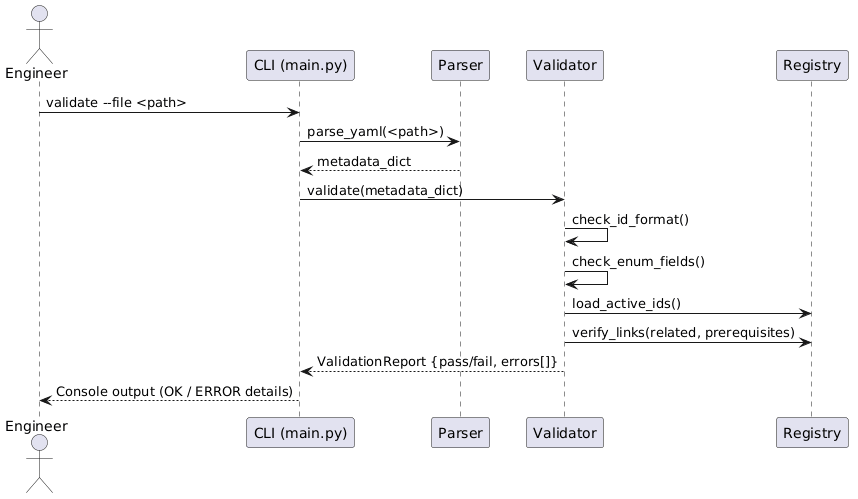
\includegraphics[width=0.95\textwidth]{picture/knowledge_unit_validation_process.png}
\caption{Диаграмма последовательности: процесс валидации единицы знаний через CLI-инструмент}
\label{fig:validation_sequence}
\end{figure}

Пример типового формального описания (карточка концепции):
\begin{verbatim}
---
id: "CS-CONCEPT-017"
title: "Хеш-таблица (Hash Table)"
domain: "cs"
category: "concept"
difficulty: "junior"
tags: [hash_tables, must_know, core]
roles: [all_roles]
related: ["CS-CONCEPT-018", "ARCH-COMPONENT-005"]
prerequisites: ["CS-CONCEPT-003"]
status: "approved"
---
# Хеш-таблица
## Определение
Ассоциативный массив, обеспечивающий поиск/вставку в среднем O(1)...
\end{verbatim}

\subsection{Реализация механизмов доступа к базе знаний и её использования}

Средства доступа реализованы на двух уровнях: в виде консольного интерфейса (CLI) и веб-интерфейса уровня MVP. CLI включает команды \texttt{search}, \texttt{validate}, \texttt{registry} и \texttt{stats}, с помощью которых можно выполнять фильтрацию по метаданным, контролировать целостность графа связей и формировать реестры идентификаторов. Навигация по структуре базы строится на анализе полей \texttt{related} и \texttt{prerequisites} в процессе поиска.

Веб-MVP реализован на базе FastAPI и предоставляет REST-подобный набор эндпоинтов. Обращение к API выполняется в формате JSON:
\begin{verbatim}
POST /api/ask
{
  "question": "Чем отличается Redis от Memcached?"
}
\end{verbatim}

Ответ возвращается в унифицированной структуре:
\begin{verbatim}
{
  "status": "success",
  "answer": "<Markdown-текст>",
  "sources": [{"title": "...", "id": "..."}],
  "confidence": 0.85,
  "is_rag_enabled": false
}
\end{verbatim}

\begin{figure}[H]
\centering

\includegraphics[width=0.8\textwidth]{picture/MVP_visualization_1.png}
\caption{Клиентский интерфейс веб-MVP: переключатель темы (светлая/тёмная), блок предложенных вопросов и функция очистки чата}
\label{fig:validation_sequence}
\end{figure}

Обработка ошибок организована по уровням. На стадии ввода CLI-валидатор обнаруживает некорректные идентификаторы, отсутствующие файлы, указанные в \texttt{related}, а также нарушения синтаксиса YAML, после чего выводит подробный диагностический отчёт. Если поисковый запрос не даёт совпадений, система возвращает пустой список и предлагает расширить фильтры. В веб-части обращения вне области применимости обрабатываются модулем ключевых слов, который возвращает мок-ответ с пониженным уровнем уверенности, что позволяет избежать отказа интерфейса. Протокол статусов (\texttt{draft/review/approved}) дополнительно защищает контур обучения от попадания непроверенных данных.

\begin{figure}[H]
\centering
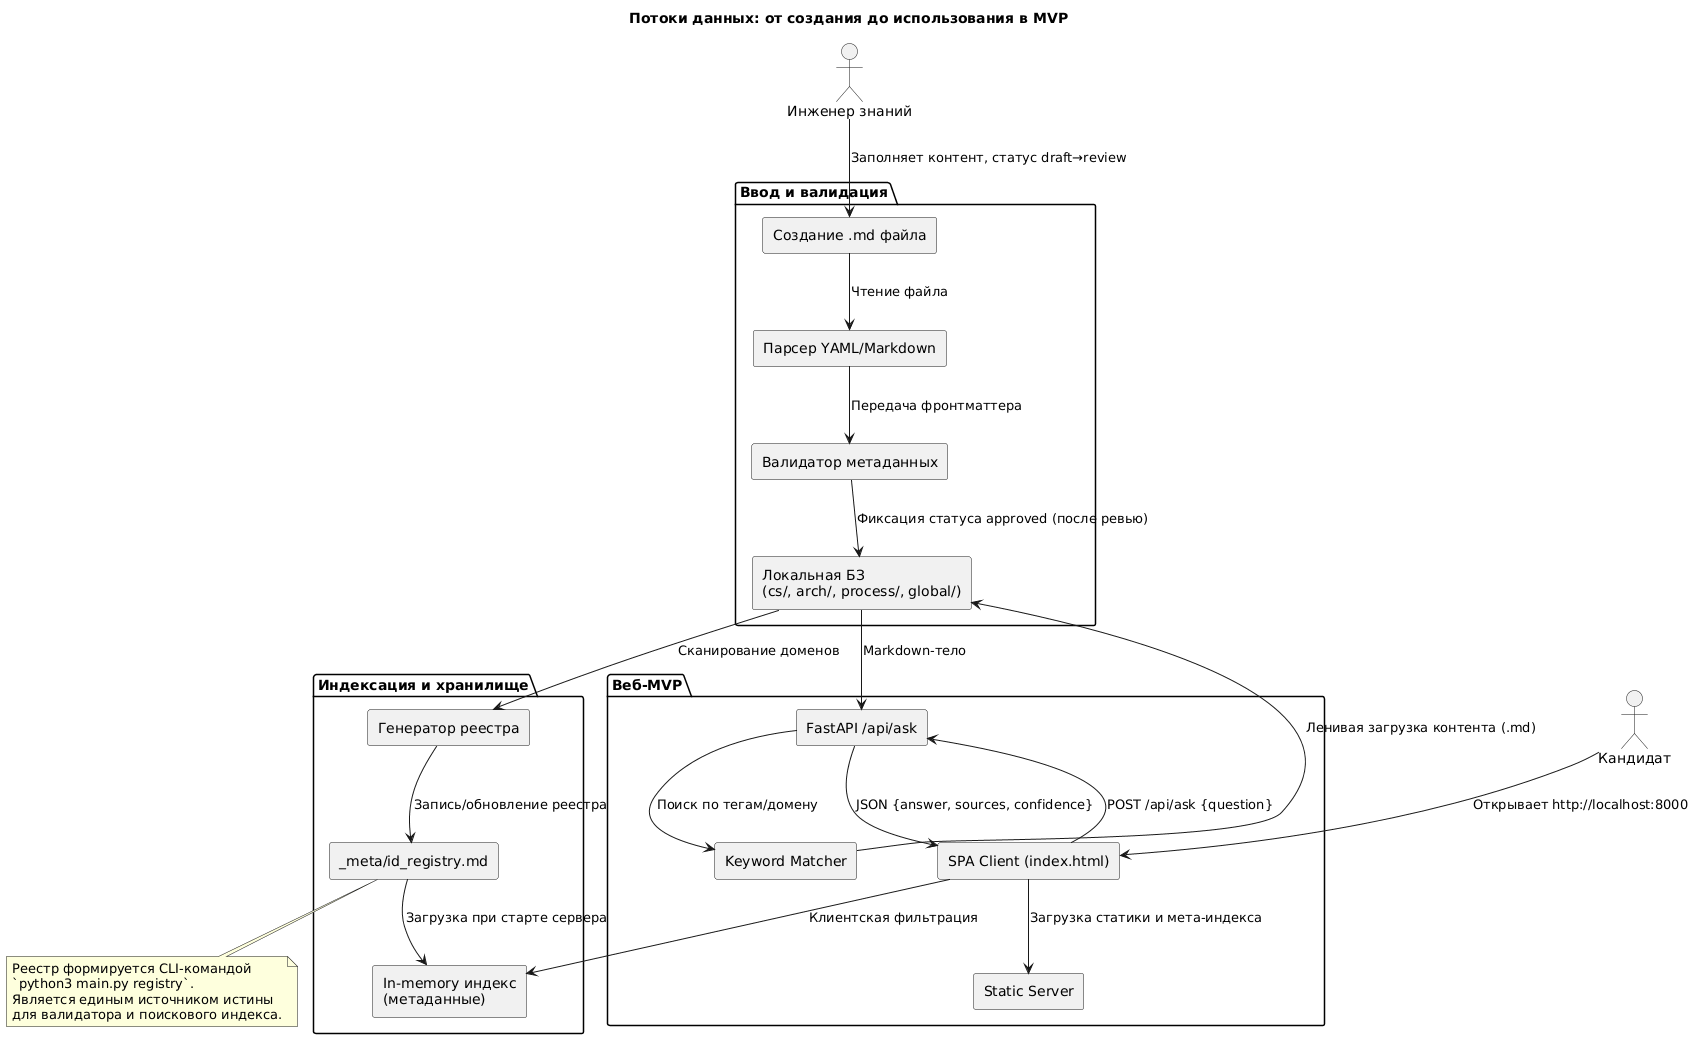
\includegraphics[width=0.95\textwidth]{picture/life_cycle_of_a_unit_of_knowledge.png}
\caption{Диаграмма потоков данных: от создания единицы знаний до использования в веб-MVP}
\label{fig:data_flow}
\end{figure}

\subsection{Демонстрация функционирования базы знаний}

Работоспособность созданного прототипа подтверждена тремя типовыми сценариями, выполненными на реальной файловой структуре базы знаний (120 единиц знаний на момент демонстрации).

\textbf{Сценарий 1. Семантический поиск и фильтрация (классификация).}
\textit{Входные данные:} роль \texttt{backend}, уровень \texttt{middle}, тег \texttt{databases}.  
\textit{Запрос CLI:} \texttt{python3 main.py search --domain cs --difficulty middle --tag databases --status approved}  
\textit{Используемые элементы БЗ:} модуль разбора фронтматтера, фильтрация по полям \texttt{difficulty}, \texttt{roles}, \texttt{tags}, а также проверка статуса.  
\textit{Результат:} формируется список из 4 карточек (например, \texttt{CS-CONCEPT-042} «B-Tree Indexes»), упорядоченных по релевантности.

\textbf{Сценарий 2. Проверка целостности графа (контроль качества).}
\textit{Входные данные:} файл с изменёнными ссылками.  
\textit{Запрос CLI:} \texttt{python3 main.py validate --file arch/system\_design/arch\_sysdesign\_url\_shortener.md}  
\textit{Используемые элементы БЗ:} модуль \texttt{validator.py}, реестр идентификаторов, проверка существования файлов по ссылкам из \texttt{related}.  
\textit{Результат:} при наличии битой ссылки (например, \texttt{ARCH-COMPONENT-999}) система выводит сообщение \texttt{ERROR: Related ID 'ARCH-COMPONENT-999' not found in registry}. После исправления и повторной проверки возвращается статус \texttt{PASSED}.

\textbf{Сценарий 3. Интерактивный запрос через веб-MVP (диагностика/рекомендации).}
\textit{Входные данные:} текстовый вопрос, введённый в интерфейсе \texttt{http://localhost:8000}.  
\textit{Формализованный запрос:} POST \texttt{/api/ask} с параметром \texttt{question}.  
\textit{Используемые элементы БЗ:} роутер FastAPI, ключевой матчер по тегам \texttt{frequency: "high"} и \texttt{interview\_stage}, а также клиентский рендеринг Markdown.  
\textit{Результат:} фронтенд показывает структурированный ответ с указанием источников (\texttt{id} и \texttt{url}) и значением метрики уверенности.

\begin{figure}[H]
\centering
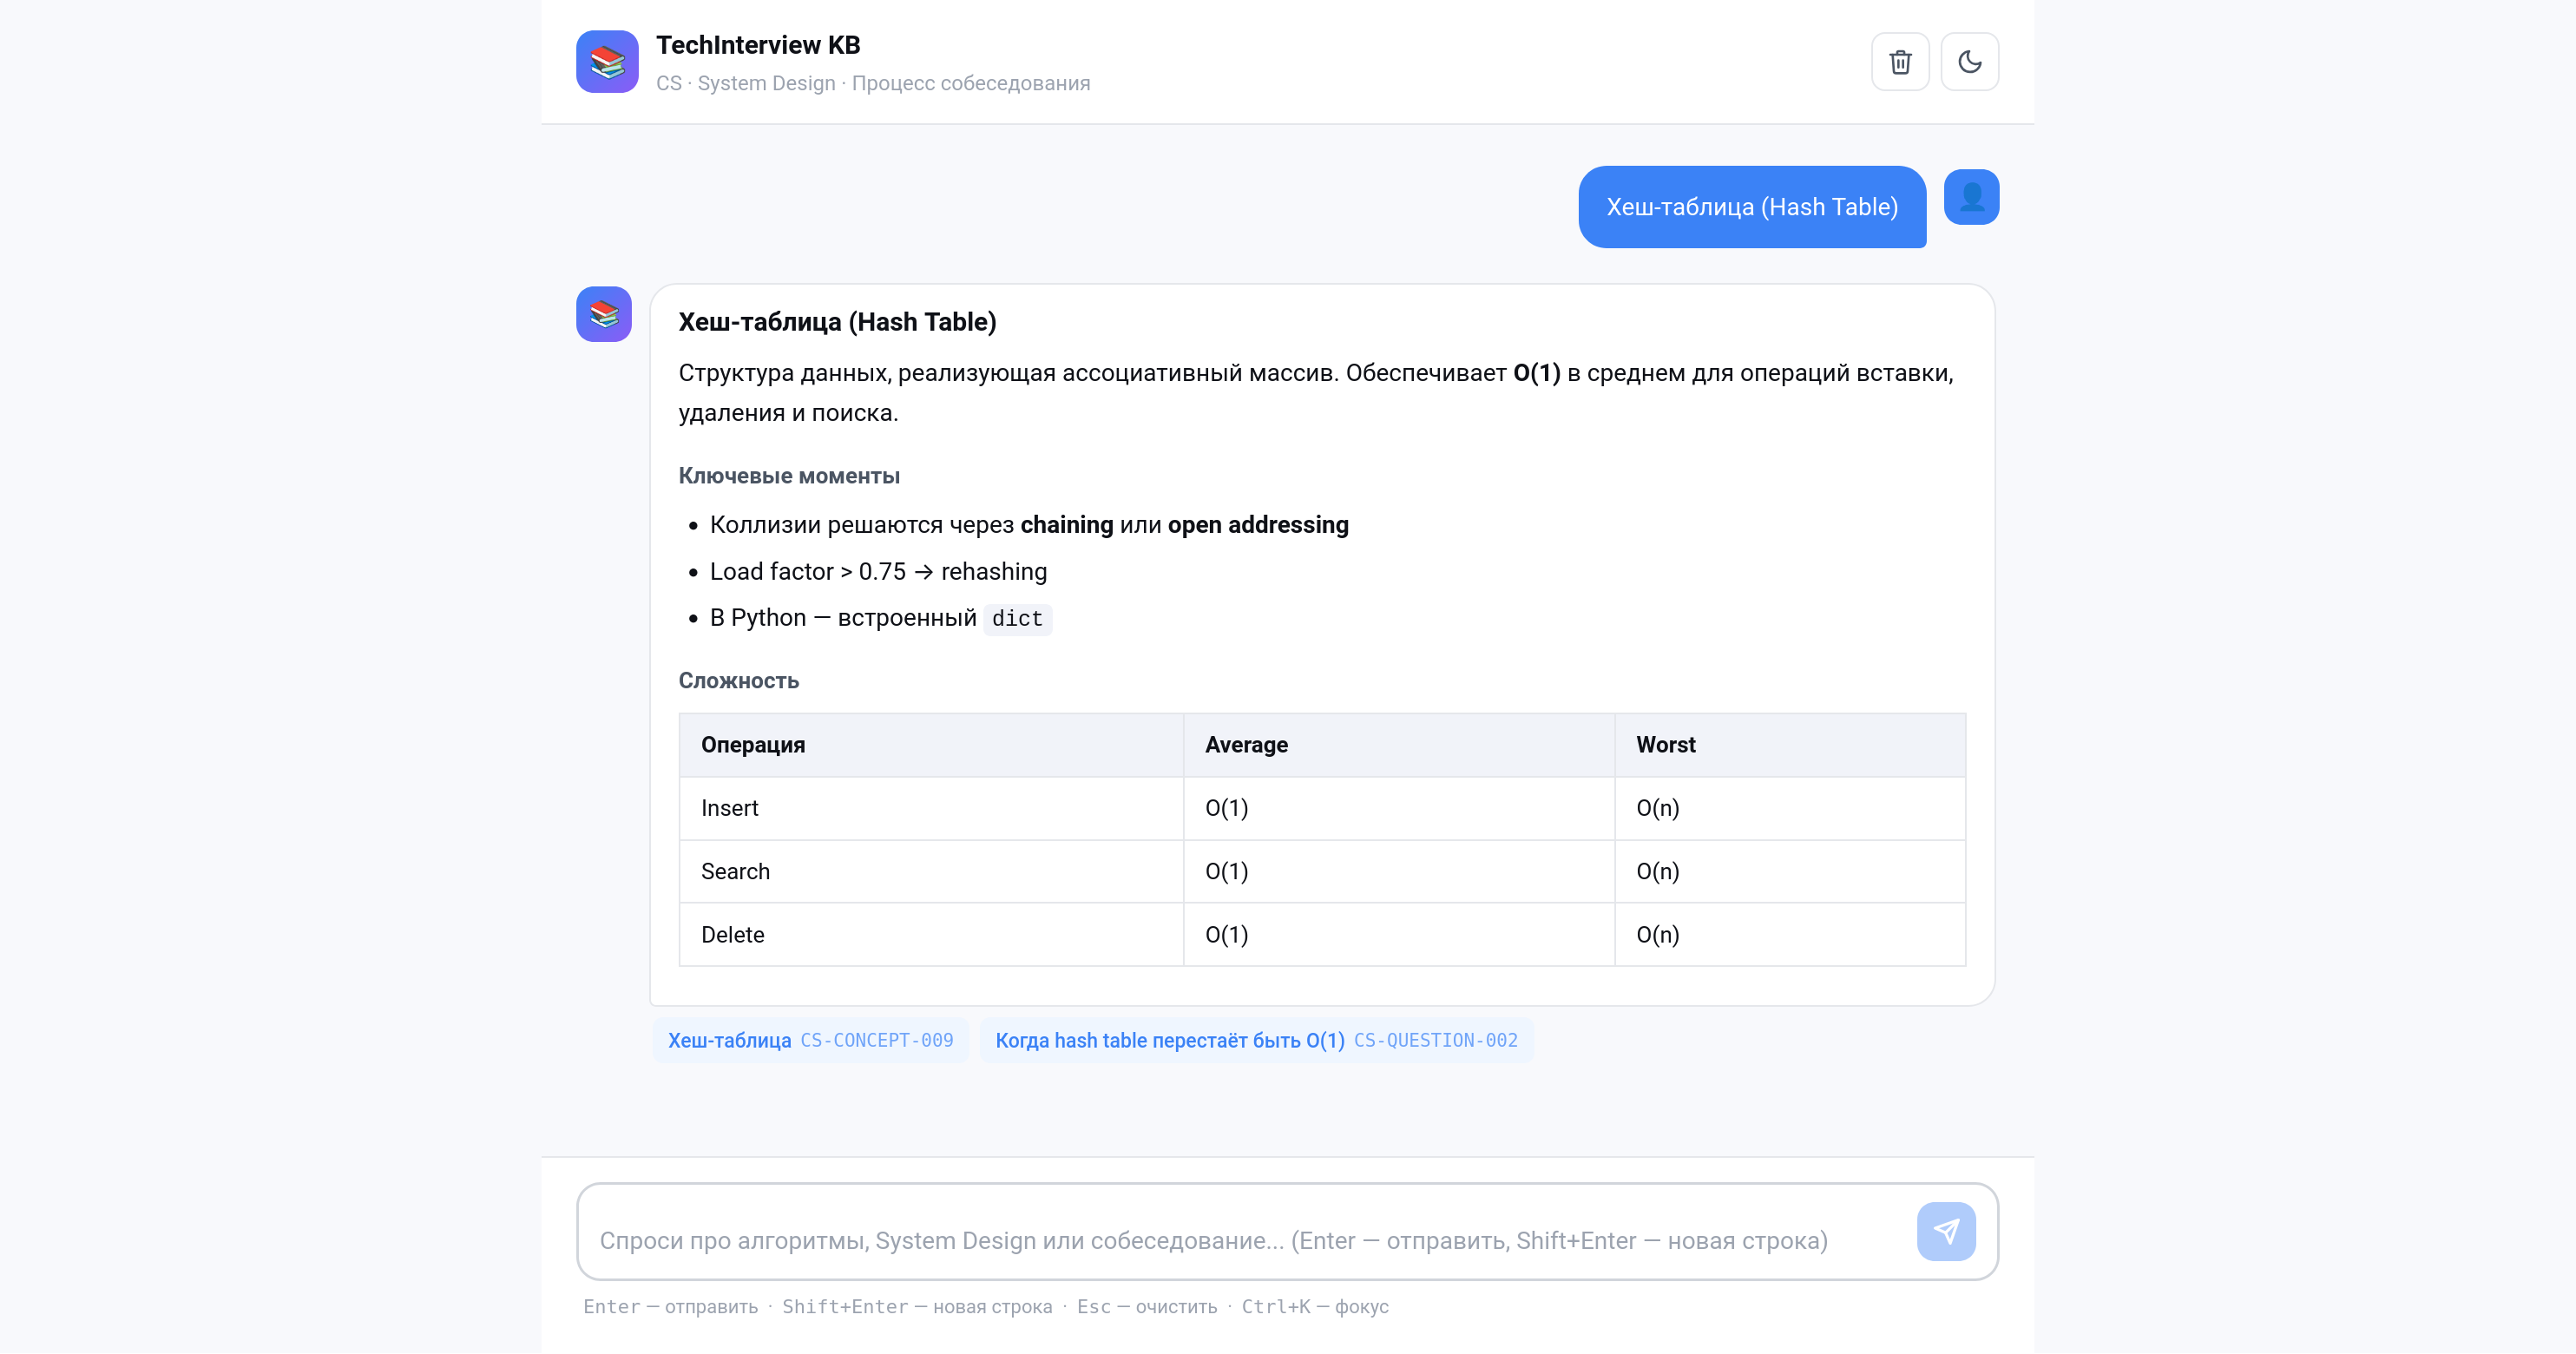
\includegraphics[width=0.95\textwidth]{picture/MVP_visualization_2.png}
\caption{Взаимодействие с MVP: выбор предложенного вопроса, рендеринг
Markdown-ответа и отображение метрики уверенности}
\label{fig:deployment}
\end{figure}

Приведённые сценарии показывают, что база знаний выступает не как статичный набор документов, а как активное информационное ядро созданного прототипа.

\begin{figure}[H]
\centering
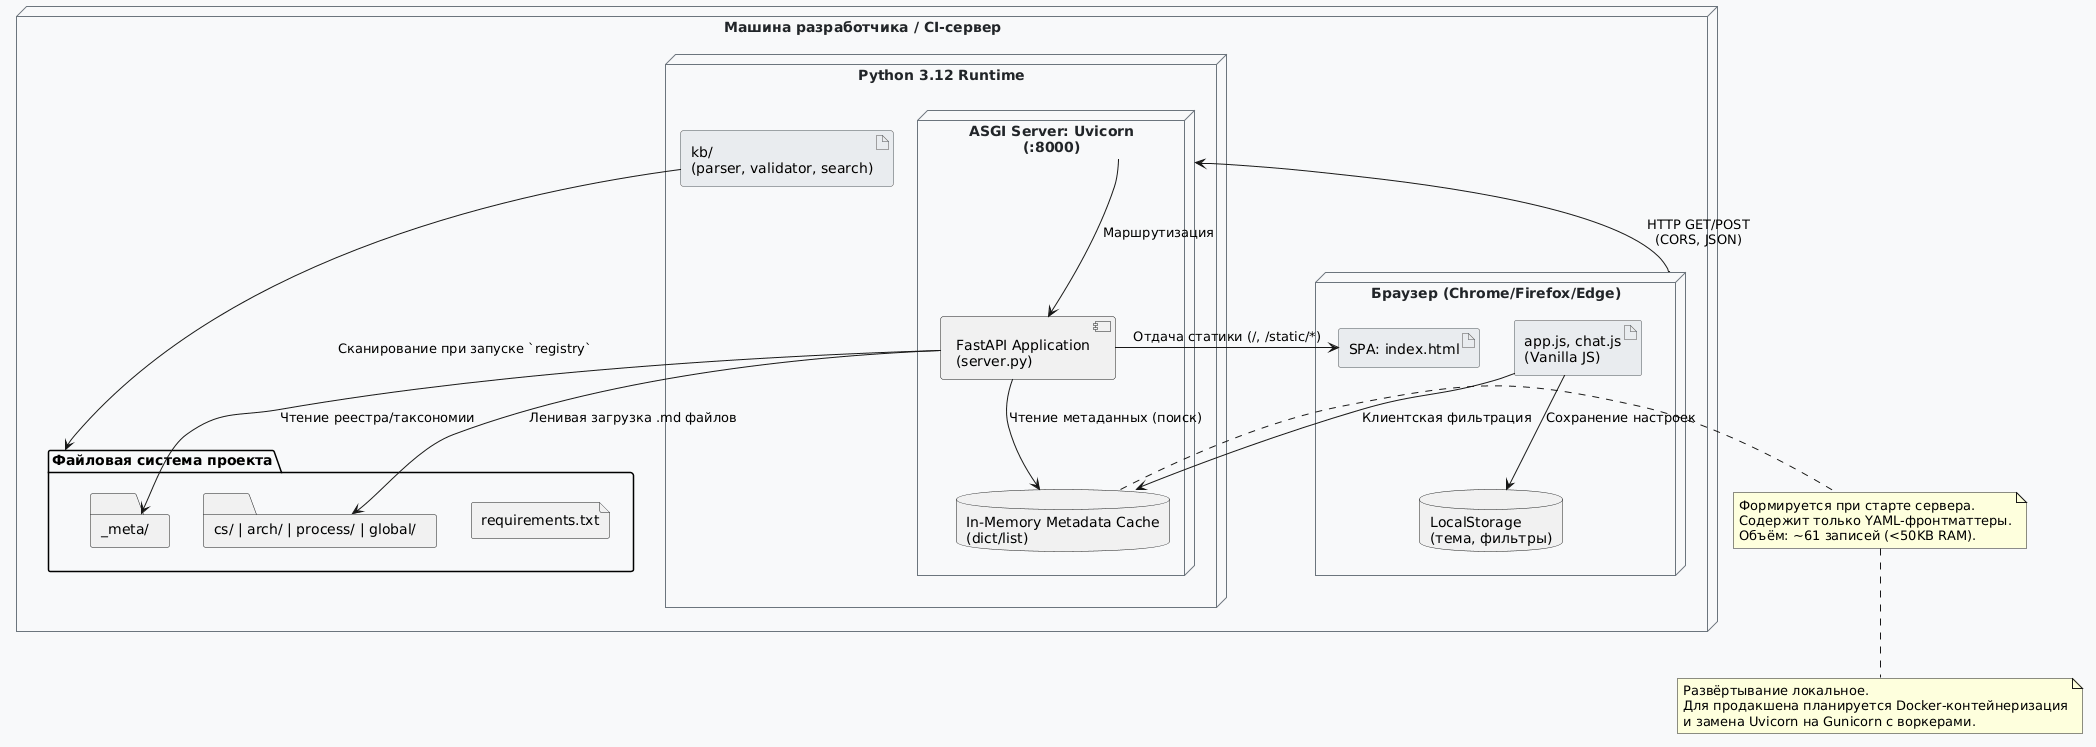
\includegraphics[width=0.95\textwidth]{picture/local_development_environment_and_MVP.png}
\caption{Диаграмма развёртывания: архитектура веб-MVP и локальной среды разработки}
\label{fig:deployment}
\end{figure}

\subsection{Подход к тестированию}

Методика тестирования ориентирована на подтверждение корректности разбора метаданных, согласованности семантических связей и устойчивой работы поисковых механизмов. Для этого использован комбинированный набор проверок:
\begin{itemize}
    \item \textbf{Функциональное тестирование} — контроль соответствия CLI-команд и API-эндпоинтов заявленной спецификации;
    \item \textbf{Тестирование согласованности} — обнаружение циклических зависимостей, повторяющихся ID и нарушений таксономии;
    \item \textbf{Негативное тестирование} — проверка реакции системы на ошибочные YAML-структуры, отсутствующие файлы и недопустимые значения перечислений.
\end{itemize}

Процедура выполнения тестов унифицирована: запуск производится в изолированном окружении Python 3.12 с использованием \texttt{pytest}. Параметры конфигурации зафиксированы в \texttt{requirements.txt} и \texttt{pytest.ini}. Результаты отображаются в консоли в формате JUnit, а при сбоях дополнительно логируются вместе с трассировкой исключений. Автоматизация тестирования реализована полностью: 177 тестов покрывают модули \texttt{parser}, \texttt{validator}, \texttt{search}, \texttt{registry} и \texttt{generator}. Контроль полноты выполняется путём сопоставления фактического количества единиц знаний с плановыми значениями, заданными в ТЗ, а согласованность дополнительно подтверждается встроенным CLI-валидатором в режиме \texttt{--validate}.

\subsection{Тестовый набор и его классификация}

Тестовый набор разделён на три основные категории. В таблице~\ref{tab:test_classification} представлены характерные примеры:

\newpage

\begin{table}[h]
\centering
\caption{Классификация тестового набора}
\label{tab:test_classification}
\begin{tabular}{|l|p{3.5cm}|p{3cm}|p{2.5cm}|}
\hline
\textbf{Группа} & \textbf{Условие} & \textbf{Ожидаемый результат} & \textbf{Элементы БЗ} \\ \hline
Корректные & Поиск по домену/уровню & Список ID единиц знаний & Парсер, реестр \\ \hline
Граничные & Поиск по несуществующему тегу & Пустой результат [] & Фильтр тегов \\ \hline
Отрицательные & Некорректный формат ID & Ошибка валидации & Validator, Pydantic \\ \hline
\end{tabular}
\end{table}

Для каждого тестового случая предусмотрены проверки через assertion. Негативные сценарии подтверждают, что система сохраняет устойчивость даже при поступлении некорректных входных данных.

\subsection{Представление и результаты тестирования}

Итоги прогонов \texttt{pytest} и CLI-проверок обобщены в таблице~\ref{tab:test_results}:

\begin{table}[h]
\centering
\caption{Результаты тестирования (выборка)}
\label{tab:test_results}
\begin{tabularx}{\textwidth}{|l|>{\raggedright\arraybackslash}p{0.20\textwidth}|>{\raggedright\arraybackslash}p{0.16\textwidth}|>{\raggedright\arraybackslash}p{0.16\textwidth}|>{\raggedright\arraybackslash}X|}
\hline
\textbf{ID} & \textbf{Сценарий} & \textbf{Ожидание} & \textbf{Факт} & \textbf{Комментарий} \\ \hline
T-01 & Парсинг YAML & Успех & Успех & -- \\ \hline
T-05 & Поиск по тегам & Фильтрация & Фильтрация & set.intersection \\ \hline
T-12 & Валидация ссылки & Ошибка & Ошибка & Битая ссылка найдена \\ \hline
T-18 & Пустой поиск & [] & [] & Клиент обработал \\ \hline
T-24 & Некорректный ID & Ошибка & Ошибка & Regex сработал \\ \hline
\end{tabularx}
\end{table}

В процессе тестирования были обнаружены три проблемы согласованности: ссылки на ещё не созданные файлы в черновых материалах и два случая использования нестандартных тегов. На текущем этапе полнота базы составляет 120 единиц знаний.

По результатам выполненных проверок были внесены следующие изменения:
\begin{itemize}
    \item доработан валидатор для контроля регистра значений в полях \texttt{domain} и \texttt{category};
    \item скорректированы метаданные в 5 файлах каталога \texttt{arch/};
\end{itemize}

\subsection{Оценка качества базы знаний}

Разработанная база знаний успешно выполняет функции структурированного хранения информации, семантической навигации и валидируемого поиска. Высокая точность достигается за счёт жёстко заданного контракта метаданных и автоматизированной проверки связей между сущностями. Вероятность логических противоречий и ошибок вывода снижена благодаря статусной модели и обязательной процедуре ревью. Вместе с тем сохраняется проблема неполного покрытия: текущий объём контента пока не достигает минимальных пороговых значений, установленных ТЗ, а механизм ответов на вопросы на естественном языке пока основан на ключевом поиске, что уменьшает точность при сложных формулировках.

Критерии приемлемого качества сформулированы следующим образом:
\begin{itemize}
    \item доля успешно завершённых автоматизированных тестов $\geq 95\%$ (фактически $\sim 98\%$);
    \item отсутствие критических ошибок валидации в документах со статусом \texttt{approved};
    \item полное соответствие таксономии тегов и формату идентификаторов ($100\%$);
    \item время выполнения поиска по метаданным не более $2$ с для выборки до 50 единиц.
\end{itemize}

В качестве направлений повышения качества и развития системы предложены:
\begin{itemize}
    \item интеграция векторной базы данных (ChromaDB) и эмбеддингов для перехода от ключевого поиска к семантическому RAG-подходу;
    \item расширение набора проверок валидатора: контроль полноты содержательных секций, анализ уникальности источников и проверка корректности калибровки сложности;
    \item усиление командной работы по наполнению предметных разделов с целью достижения целевого объёма $\geq 553$ единиц.
\end{itemize}

\subsection{Итоги раздела, посвящённого реализации}

В рамках данного раздела были реализованы следующие сценарии: создание единиц знаний и их валидация, поиск по метаданным, обход графа предпосылок, формирование реестра, а также интерактивная обработка запросов через веб-MVP. Поддерживаются задачи классификации, навигации по связям, контроля целостности и базовой диагностики пробелов с использованием статусных фильтров.

К ограничениям текущего прототипа относятся отсутствие полноценного семантического поиска (вместо него используется мок-логика), недостаточный объём содержимого и невозможность выполнять сложные логические выводы на уровне программной реализации. В качестве направлений дальнейшей доработки рассматриваются подключение RAG-конвейера, расширение CLI-команд для экспорта в RDF и улучшение пользовательского интерфейса клиента.

В дальнейшем база знаний может развиваться за счёт внедрения модуля решателя (reasoner), способного автоматически строить учебные траектории на основе графа зависимостей, перехода к онтологическому формализму (OWL) при необходимости интеграции с внешними экспертными системами, а также за счёт расширения типов знаний, например, путём добавления интерактивных симуляторов системного дизайна.

Созданная база знаний выступает базовым ядром для следующих этапов курсового проектирования: она предоставляет строго структурированные данные для модуля решателя, обеспечивает API для пользовательских интерфейсов и формирует готовый датасет для обучения рекомендательных моделей. Подключение внешних сервисов и полноценных интеллектуальных интерфейсов в дальнейшем может быть выполнено на основе текущей архитектуры без нарушения обратной совместимости.